\documentclass{article}

\usepackage{pgfplots}
\usepackage[left=1cm]{geometry}

\pgfplotsset{compat=1.13}
\usepgfplotslibrary{patchplots}

\begin{document}

\parskip=20pt
\parindent=0pt


\def\PLOTx[#1]{%
	\addplot[point meta=explicit,#1]
	coordinates {
	(0,0) [\pgfkeysvalueof{/CC/00}] (1,0) [\pgfkeysvalueof{/CC/10}] (2,0) [\pgfkeysvalueof{/CC/20}]

	(0,1) [\pgfkeysvalueof{/CC/01}] (1,1) [\pgfkeysvalueof{/CC/11}] (2,1) [\pgfkeysvalueof{/CC/21}]

	(0,2) [\pgfkeysvalueof{/CC/02}] (1,2) [\pgfkeysvalueof{/CC/12}] (2,2) [\pgfkeysvalueof{/CC/22}]
	};
}%

\pgfkeys{
	/c/none/.initial=,
	/c/00/.initial={color=red},
	/c/10/.initial={color=blue},
	/c/20/.initial={color=yellow},
	%
	/c/01/.initial={color=black},
	/c/11/.initial={color=brown},
	/c/21/.initial={color=magenta},
	%
	/c/02/.initial={color=green},
	/c/12/.initial={color=red},
	/c/22/.initial={color=gray},
	%
	%
	%
	/CC/none/.initial=,
	/CC/00/.initial={0},
	/CC/10/.initial={1},
	/CC/20/.initial={2},
	%
	/CC/01/.initial={3},
	/CC/11/.initial={4},
	/CC/21/.initial={5},
	%
	/CC/02/.initial={6},
	/CC/12/.initial={7},
	/CC/22/.initial={8},
	%
}
\def\PLOT[#1]{%
	\addplot[point meta=explicit symbolic,mesh/color input=explicit,#1]
	coordinates {
	(0,0) [\pgfkeysvalueof{/c/00}] (1,0) [\pgfkeysvalueof{/c/10}] (2,0) [\pgfkeysvalueof{/c/20}]

	(0,1) [\pgfkeysvalueof{/c/01}] (1,1) [\pgfkeysvalueof{/c/11}] (2,1) [\pgfkeysvalueof{/c/21}]

	(0,2) [\pgfkeysvalueof{/c/02}] (1,2) [\pgfkeysvalueof{/c/12}] (2,2) [\pgfkeysvalueof{/c/22}]
	};
}%


	\subsection{multiple cells}
	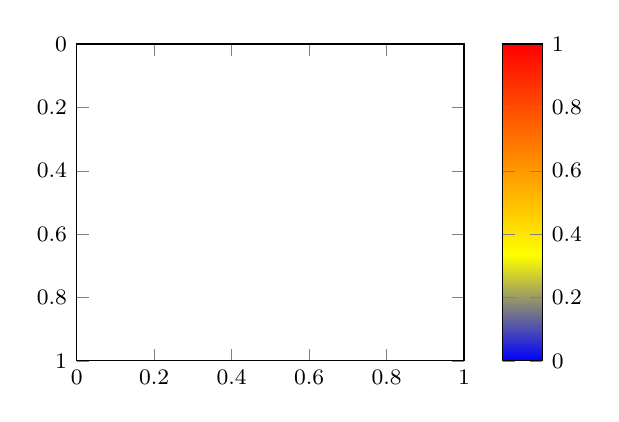
\begin{tikzpicture}
		%\tracingmacros=2 \tracingcommands=2
		\begin{axis}[
			small,
			colorbar,
			axis on top,
			y dir=reverse,
			enlargelimits=false,
			shader=flat corner,
			patch type=bilinear,
		]

		\PLOT[surf, mesh input=image,
			/c/00={},
			/c/11={},
			/c/20={},
		]

		\PLOT[mark=*,%scatter,
			mark size=4pt,only marks]
			
		\end{axis}
	\end{tikzpicture}

	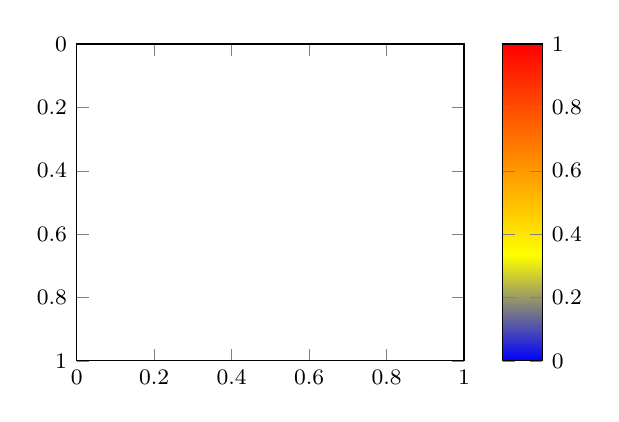
\begin{tikzpicture}
		%\tracingmacros=2 \tracingcommands=2
		\begin{axis}[
			small,
			colorbar,
			axis on top,
			y dir=reverse,
			enlargelimits=false,
			shader=flat corner,
			patch type=bilinear,
		]

		\PLOTx[surf, mesh input=image,
			/CC/01={nan},
			/CC/11={nan},
			/CC/22={nan},
		]

		\PLOTx[mark=*,scatter,
			mark size=4pt,only marks]
			
		\end{axis}
	\end{tikzpicture}
\end{document}

